%!TEX root = ../dokumentation.tex

\chapter{Grundlagen der Arbeit}

Im Folgenden werden die zu Grunde liegenden Technologien der Arbeit kurz erörtert.
%title wird unter dem Bsp. abgedruckt
%caption wird im Verzeichnis abgedruckt
%label wird zum referenzieren benutzt, muss einzigartig sein.

\section{Raspberry Pi 3 Model B}
Ein \textit{Raspberry Pi} ist ein kleiner Minicomputer, welcher in etwa die
Größe einer Kreditkarte einnimmt. Seit der Erstveröffentlichung im Jahre 2011
hat sich am Grundkonzept des kleinen Computers nicht viel
geändert, lediglich die Anschlüsse sind mehr geworden und die verbauten
Prozessoren haben sich verbessert. 
Ein Grund für die weite Verbreitung der Minicomputer ist neben der kleinen
Größe auch der günstige Preis. So liegt der Preis des aktuellsten Modells bei
gerade einmal 30 Euro. Des Weiteren ist der Stromverbrauch sehr gering,
weshalb der Raspberry von den Benutzern auch oft als kleiner Server im Heimnetz
betrieben wird. Im Dauerbetrieb liegt dieser beim neusten Raspberry
Pi's 3 Modell B aufs Jahr gerechnet etwa bei 53 kWh, was bei einem Preis von
circa 20 Cent pro kWh Gesamtkosten von 10 Euro pro Jahr bedeuten würde. \newline
Die Intention der Entwickler war es mit dem Raspberry Pi ein Gerät zu
entwerfen, welches Personen in jedem Alter die Möglichkeit bietet einen
Computer zu benutzen und programmieren zu lernen. Das Standard Betriebssystem
des Raspberry Pi basiert auf einer eigen entwickelten Linux Distribution mit
dem Namen \textit{Raspbian}.
\autocite{what_is_a_raspberry_pi?_2019}
\begin{figure}[h]
	\centering
	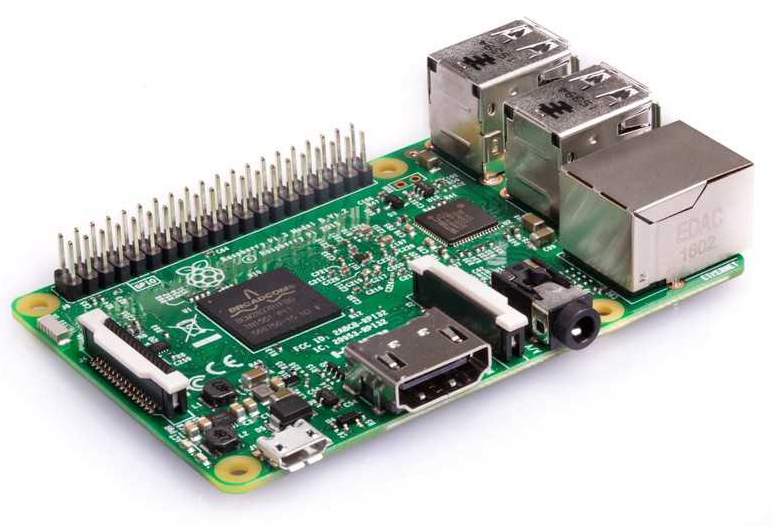
\includegraphics[scale=0.35]{Raspberry_Pi_3_Model_B.jpg}
	\caption{Beispielbild - Raspberry Pi 3 Model B \autocite{raspberry_pi_2019}}
	\label{img:grafik-RaspberryPi3}
\end{figure}
\newline

Auf dem in der Abbildung \ref{img:grafik-RaspberryPi3} dargestellten Raspberry
Pi handelt es sich um ein Gerät der neusten Generationen, den Raspberry Pi 3
Model B. Er zeichnet sich durch eine neue 64-Bit \ac{ARM}-\ac{CPU} mit 1.2
\ac{GHz} aus und besitzt dazu 1 \ac{GB} \ac{RAM}. Des Weiteren stellt er
sämtliche Anschlüsse wie z.B. 4 \ac{USB} Ports, RJ45 Anschluss, \ac{HDMI}
Anschluss sowie 40 \ac{GPIO} Ports zur Verfügung. Mit dem neusten Model des
Raspberry Pi wurde zudem noch eine \ac{WLAN} sowie Bluetooth Karte integriert.
In der Kombination mit dem \ac{SD-Karten} Slot, welcher als Speicher benutzt
wird, stellt der Raspberry Pi einen vollwertigen Computer dar.
\autocite{kurniawan_2016}
 
\section{Go}
\textit{Go} (oder auch\textit{Golang}) ist eine Programmiersprache, welche von
Robert Griesemer, Rob Pike und Ken Thompson entwickelt wurde (alles Mitarbeiter
von Google). Ziel hinter Go war es eine effiziente und ausdrucksstarke Sprache zu entwickeln, welche es ermöglicht verlässliche und
leicht-leserliche Programme zu entwerfen \autocite{donovan_kernighan_2016}.
2009 wurde Go erstmals veröffentlicht, und wird seitdem von Google als Open Source
Software veröffentlicht. \newline
Im Vergleich zu anderen Programmiersprachen reiht sich Go zwischen C/C++ und
Perl ein. Google legt einen großen Wert darauf, Go als Sprache für die
Systemprogrammierung zu positionieren, setzt dazu aber nicht typische Mittel
wie einen Garbage Collector oder die Unterstützung zur Parallel- und
Multicore-Verarbeitung ein \autocite{feike_blass_2012}. Go überzeugt die Nutzer
durch seine Einfachheit beim der Programmierung sowie durch die Geschwindigkeit beim
der Kompilierung und Ausführung des Codes. Zusätzlich wird die Nebenläufigkeit von
Prozessen unterstützt, die \textit{Goroutinen} genannt werden und über Kanäle
miteinander kommunizieren können. 
Ein weiterer großer Vorteil ist, dass Go plattformübergreifend läuft. Das heißt,
dass Go ohne weitere Modifikation auf jedem gängigen Betriebssystem gleich
läuft.
\autocite{donovan_kernighan_2016}


\section{Git and GitHub}
\textit{Git} ist eines der bekanntesten Versionskontrollsysteme welches 2005
von Linus Torvalds entwickelt wurde. Unter einem Versionskontrollsystem wird
ein Software verstanden, die die Veränderung von Dateien über einen Zeitraum
aufzeichnet und speichert. Dadurch wird es auch ermöglicht zu jedem Zeitpunkt
wieder auf einen alten Dateizustand zurückzuspringen.  Genauer genommen ist
\textit{Git} ein verteiltest Versionskontrollsystem, was bedeutet dass alle
Personen in einem  Projekt nicht nur den aktuellen Stand sondern auch die
komplette Historie einsehen können. \autocite{preissel_stachmann_2017}
\newline
\newline
\textit{GitHub} ist eine Webseite in der man eine Kopie eines \textit{Git}
Repository speichern kann. Dadurch ergibt sich ein zentralisierter Ort um
einfach mit anderen Personen an einem Projekt  arbeiten zu können.
\textit{GitHub} bietet vor allen Dingen durch seine weiteren Funktionen wie
z.B. ein Web Interface, ein Wiki sowie einen Bereich zum diskutieren und
bewerten von Änderungen, eine ausgewogene Arbeitsumgebung zum Entwickeln von
Software. \autocite{bell_2014}
